\documentclass{beamer}
\usepackage[utf8]{inputenc}
\usepackage{graphicx, epsfig}
\usepackage{amsmath,mathrsfs,amsfonts,amssymb}
\usepackage{subfig}
\usepackage{floatflt}
\usepackage{epic,ecltree}
\usepackage{mathtext}
\usepackage{fancybox}
\usepackage{fancyhdr}
\usepackage{multirow}
\usepackage{enumerate}
\usepackage{epstopdf}
\usepackage{multicol}
\usetheme{Boadilla}%{Singapore}%{Warsaw}%{Warsaw}%{Darmstadt}
\usecolortheme{beaver}
%\definecolor{beamer@blendedblue}{RGB}{15,120,80}
%----------------------------------------------------------------------------------------------------------
\title[\hbox to 56mm{Matrix Completion  \hfill\insertframenumber\,/\,\inserttotalframenumber}]
{Low-Rank Matrix Completion project}
\author[ROY team]{\\
				{\small \textbf{Authors:} Artem Bochkarev, Roman Isachenko \\
					 Ilya Zharikov, Anne-Laure Ducrocq}}
\institute[SkolTech]{Skolkovo Institute of Science and Technology \\
	Methods of Optimization course 
    \vspace{0.3cm}
}
\date{December 16, 2016.}
%--------------------------------------------------------------------------------
\begin{document}
%--------------------------------------------------------------------------------
\begin{frame}
%\thispagestyle{empty}
\titlepage
\end{frame}
%--------------------------------------------------------------------------------
\begin{frame}{Problem Statement}
\begin{block}{Task}	
	Given the amount of observed matrix entries to reconstruct low-rank matrix approximation.
\end{block}
\vspace{0.3cm}
\textbf{Applications:}
\begin{itemize}
	\item  recommender systems;
	\item image-processing;
	\item imputation of NAs for genomic data;
	\item rank estimation for SVD.
\end{itemize}
\end{frame}
%--------------------------------------------------------------------------------
\begin{frame}{Problem Statement}
\textbf{Notations:}
\begin{itemize}
	\item $M$~--- $n \times m$ unknown matrix;
	\item $\Omega \in \{1, \dots, n\} \times \{1, \dots, m\}$ indices of observed elements;
	\item 
	$$
	P_{\Omega} (M) = 
	\begin{cases}
	M_{ij}, &\text{if} \, (i, j) \in \Omega;\\
	0, &\text{otherwise}.
	\end{cases}
	$$
\end{itemize}
\begin{block}{Optimization Task ($NP-hard$)}
	\vspace{-0.5cm}
	\begin{align*}
		\mathop{\text{minimize}}\limits_{X \in \mathbb{R}^{n \times m}} \quad & 
		\text{rank} (X) \\
		\text{subject to} \quad & P_{\Omega} (X) = P_{\Omega} (M)
	\end{align*}
\end{block}
\end{frame}
%--------------------------------------------------------------------------------
\begin{frame}{Related Works}
\begin{enumerate}
	\item Candes E. J., Recht B. Exact matrix completion via convex optimization. 2009.
	\item Cai J. F., Candes E. J., Shen Z. A singular value thresholding algorithm for matrix completion. 2010.
	\item Mazumder R., Hastie T., Tibshirani R. Spectral regularization algorithms for learning large incomplete matrices. 2010.
	\item Jain P., Meka R., Dhillon I. S. Guaranteed rank minimization via singular value projection. 2010.
	\item Takacs G. et al. Scalable collaborative filtering approaches for large recommender systems. 2009.
	\item Vandereycken B. Low-rank matrix completion by Riemannian optimization. 2013.
\end{enumerate}
\end{frame}
%--------------------------------------------------------------------------------
\begin{frame}{Convex Relaxation (Candes E. J., Recht B., 2009)}  \begin{columns}[c]
	\column{0.49\textwidth}
	\begin{block}{Original Task}
		\vspace{-0.5cm}
		\begin{align*}
		\mathop{\text{minimize}}\limits_{X \in \mathbb{R}^{n \times m}} \quad & 
		\text{rank} (X) \\
		\text{subject to} \quad & P_{\Omega} (X) = P_{\Omega} (M)
		\end{align*}
	\end{block}
	
	\column{0.49\textwidth}
	\begin{block}{Relaxation}
		\vspace{-0.5cm}
		\begin{align*}
		\mathop{\text{minimize}}\limits_{X \in \mathbb{R}^{n \times m}} \quad & 
		\| X \|_* \\
		\text{subject to} \quad & P_{\Omega} (X) = P_{\Omega} (M)
		\end{align*}
	\end{block}
\end{columns}
\vspace{0.3cm}
\textbf{Motivation:} (analogue for $l_0$ and $l_1$ regularizations)
$$
	\text{rank} (X) = |\{ i: \sigma_i(X) \neq 0\}|  \hspace{2.5cm} 
	\| X \|_* = \sum_{i=1}^{k} \sigma_i(X)
$$
\textbf{Problems:}
\begin{itemize}
	\item expensive computations;
	\item only for small matrices.
\end{itemize}
\end{frame}
%--------------------------------------------------------------------------------
\begin{frame}{SVP (Jain P., Meka R., Dhillon I. S., 2010)}
\begin{columns}[c]
	\column{0.49\textwidth}
	\begin{block}{Original Task}
		\vspace{-0.5cm}
		\begin{align*}
		\mathop{\text{minimize}}\limits_{X \in \mathbb{R}^{n \times m}} \quad & 
		\text{rank} (X) \\
		\text{subject to} \quad & P_{\Omega} (X) = P_{\Omega} (M)
		\end{align*}
	\end{block}
	
	\column{0.49\textwidth}
	\begin{block}{Relaxation}
		\vspace{-0.5cm}
		\begin{align*}
		\mathop{\text{minimize}}\limits_{X \in \mathbb{R}^{n \times m}} \quad & 
		\| P_{\Omega} (X) - P_{\Omega} (M) \|_F^2 \\
		\text{subject to} \quad & \text{rank} (X) \leq k
		\end{align*}
	\end{block}
\end{columns}
\vspace{0.3cm}
\textbf{Steps}

\begin{itemize}
	\item gradient descent  for convex function;
	\item $SVD$ projection on the $k$-dimensional space;
\end{itemize}
\textbf{Features:}
\begin{itemize}
	\item sensitive to given rank $k$;
	\item guaranteed rank minimization for $RIP$-matrices.
\end{itemize}

\end{frame}
%--------------------------------------------------------------------------------
\begin{frame}{SVT (Cai J. F., Candes E. J., Shen Z., 2010)}
	\begin{columns}[c]
		\column{0.49\textwidth}
		\begin{block}{Original Task}
			\vspace{-0.5cm}
			\begin{align*}
			\mathop{\text{minimize}}\limits_{X \in \mathbb{R}^{n \times m}} \quad & 
			\text{rank} (X) \\
			\text{subject to} \quad & P_{\Omega} (X) = P_{\Omega} (M)
			\end{align*}
		\end{block}
		
		\column{0.49\textwidth}
		\begin{block}{Relaxation}
			\vspace{-0.5cm}
			\begin{align*}
			\mathop{\text{minimize}}\limits_{X \in \mathbb{R}^{n \times m}} \quad & \tau \| X \|_* + \| X \|_F^2 \\
			\text{subject to} \quad & P_{\Omega} (X) = P_{\Omega} (M)
			\end{align*}
		\end{block}
	\end{columns}
	\vspace{0.3cm}
	\textbf{Steps}
	
	\begin{itemize}
		\item proximal gradient descent method;
		\item soft-thresholding for singular values.
	\end{itemize}
	\textbf{Features:}
	\begin{itemize}
		\item sensitive to noise;
		\item robust to matrix rank.
	\end{itemize}
	
\end{frame}
%--------------------------------------------------------------------------------
\begin{frame}{SoftImpute (Hastie T., Tibshirani R., 2010)}
	\begin{columns}[c]
		\column{0.49\textwidth}
		\begin{block}{Original Task}
			\vspace{-0.5cm}
			\begin{align*}
			\mathop{\text{minimize}}\limits_{X \in \mathbb{R}^{n \times m}} \quad & 
			\text{rank} (X) \\
			\text{subject to} \quad & P_{\Omega} (X) = P_{\Omega} (M)
			\end{align*}
		\end{block}
		
		\column{0.49\textwidth}
		\begin{block}{Relaxation}
			\vspace{-0.5cm}
			\begin{align*}
			\mathop{\text{minimize}}\limits_{X \in \mathbb{R}^{n \times m}} \quad & 
			\| X \|_* \\
			\text{subject to} \, & \| P_{\Omega} (X) - P_{\Omega} (M) \|_F \leq \delta
			\end{align*}
		\end{block}
	\end{columns}
\vspace{0.3cm}
\textbf{Motivation:}
	
	The method is the same as $SVT$ with $\delta = 0$. When $\delta>0$ the overfitting is less possible.
	
\vspace{0.3cm}
\textbf{Steps:}
\begin{itemize}
	\item proximal gradient descent method;
	\item soft-thresholded $SVD$;
	\item warm starts.
\end{itemize}

\end{frame}
%--------------------------------------------------------------------------------
\begin{frame}{RISMF}
	\begin{columns}[c]
		\column{0.49\textwidth}
		\begin{block}{Original Task}
			\vspace{-0.5cm}
			\begin{align*}
			\mathop{\text{minimize}}\limits_{X \in \mathbb{R}^{n \times m}} \quad & 
			\text{rank} (X) \\
			\text{subject to} \quad & P_{\Omega} (X) = P_{\Omega} (M)
			\end{align*}
		\end{block}
		
		\column{0.49\textwidth}
		\begin{block}{Relaxation}
			\vspace{-0.5cm}
			\begin{align*}
			\mathop{\text{minimize}}\limits_{\substack{	U \in \mathbb{R}^{n \times k} \\ V \in \mathbb{R}^{k \times m}}} \quad & \| U \|^2_F + \| V \|^2_F \\
			\text{subject to} \quad &  P_{\Omega} (UV) = P_{\Omega} (M) 
			\end{align*}
		\end{block}
	\end{columns}
	\vspace{0.3cm}
	\textbf{Steps:}
	\begin{itemize}
		\item incremental gradient descent;
		\item updating $U$ and $V$ simultaneously.
	\end{itemize}	
	\vspace{0.3cm}
	\textbf{Features:}
	\begin{itemize}
		\item need to choose learning rate;
		\item sensitive to regularization factor.
	\end{itemize}

\end{frame}
%--------------------------------------------------------------------------------
\begin{frame}{Numerical Experiments}
\begin{itemize}
	\item Synthetic data
	
	Low-rank matrices with random noise.
	\item Low-rank images
	
	Visual demonstration of algorithms.
	\item Assessment dataset
	
	Real dataset for collaborating filtering.
\end{itemize}

\end{frame}
%--------------------------------------------------------------------------------
\begin{frame}{Synthetic Data}
	\begin{figure}[h]
		\centering
		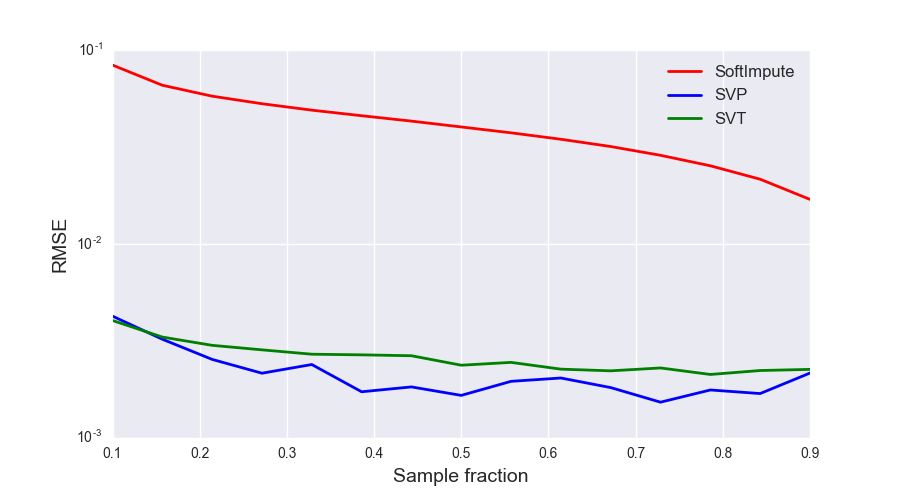
\includegraphics[width=1\linewidth]{./../results/synthetic/exper_1/synthetic_nsamp_rmse.png}
		\label{heat_map}
	\end{figure}
\end{frame}
%--------------------------------------------------------------------------------
\begin{frame}{Synthetic Data}
	\begin{figure}[h]
		\centering
		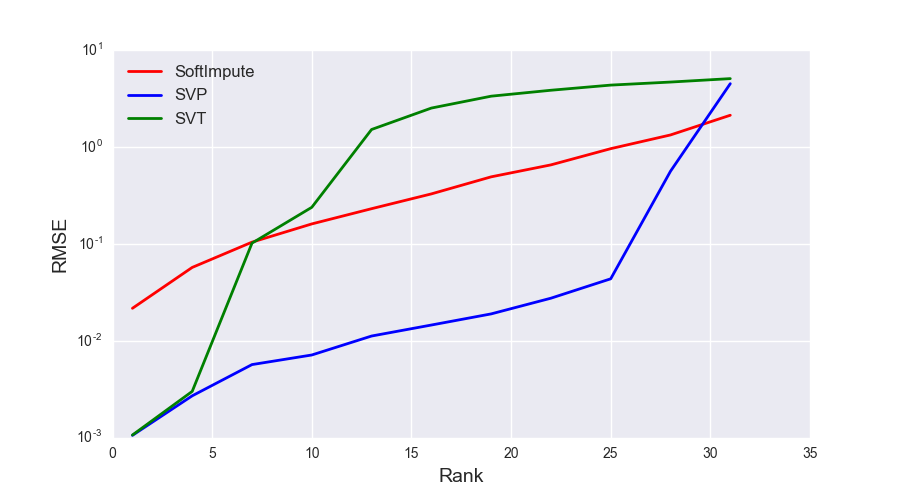
\includegraphics[width=1\linewidth]{./../results/synthetic/exper_2/synthetic_rank_rmse.png}
		\label{heat_map}
	\end{figure}
\end{frame}
%--------------------------------------------------------------------------------
\begin{frame}{Synthetic Data}
	\begin{figure}[h]
		\centering
		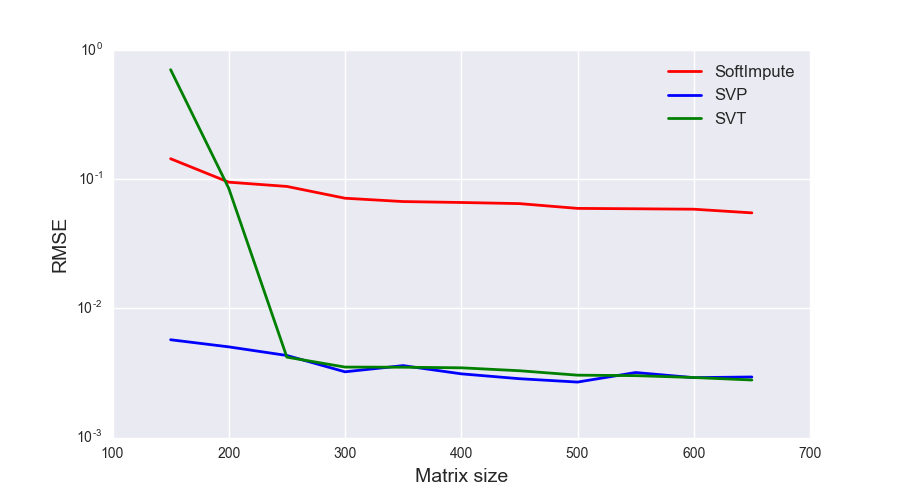
\includegraphics[width=1\linewidth]{./../results/synthetic/exper_3/synthetic_size_rmse.png}
		\label{heat_map}
	\end{figure}
\end{frame}
%--------------------------------------------------------------------------------
\begin{frame}{Images}
	\vspace{-0.2cm}
	\begin{multicols}{2}
		\hspace{0.7cm}Sampled Image
		\vspace{-0.2cm}
		\begin{figure}[h]
			\centering
			
\includegraphics[width=0.8\linewidth]{./../data/images/presentation/p1_2_01_20.jpg}
		\end{figure}
		\hspace{0.7cm}SoftImpute
		\vspace{-0.2cm}
		\begin{figure}[h]
			\centering
			
\includegraphics[width=0.8\linewidth]{./../data/images/presentation/p1_5_20_01_SI_RMSE_006935.jpg}
		\end{figure}
	\end{multicols}
	
	\vspace{-0.2cm}
	\begin{multicols}{3}
		\vspace{-0.2cm}
		\hspace{0.5cm}RISMF
		\vspace{-0.2cm}
		\begin{figure}[h]
			\centering
			
\includegraphics[width=0.8\linewidth]{./../data/images/presentation/p1_3_20_01_RISMF_RMSE_037643.jpg}
		\end{figure}
		\vspace{-0.2cm}
		\hspace{0.5cm}SVT
		\vspace{-0.2cm}
		\begin{figure}[h]
			\centering
			
\includegraphics[width=0.8\linewidth]{./../data/images/presentation/p1_3_20_01_SVT_RMSE_007624.jpg}
		\end{figure}
		\vspace{-0.2cm}
		\hspace{0.5cm}SVP
		\vspace{-0.2cm}
		\begin{figure}[h]
			\centering
			
\includegraphics[width=0.8\linewidth]{./../data/images/presentation/p1_4_20_01_SVP_RMSE_023253.jpg}
		\end{figure}
	\end{multicols}
	
\end{frame}%--------------------------------------------------------------------------------
\begin{frame}{Images}
	\vspace{-0.2cm}
	\begin{multicols}{2}
		\hspace{0.7cm}Sampled Image
		\vspace{-0.2cm}
		\begin{figure}[h]
			\centering
			
\includegraphics[width=0.8\linewidth]{./../data/images/presentation/p4_2_01_20.jpg}
		\end{figure}
		\hspace{0.7cm}SVT
		\vspace{-0.2cm}
		\begin{figure}[h]
			\centering
			
\includegraphics[width=0.8\linewidth]{./../data/images/presentation/p4_2_01_20.jpg}
		\end{figure}
	\end{multicols}
	
	\vspace{-0.2cm}
	\begin{multicols}{3}
		\vspace{-0.2cm}
		\hspace{0.5cm}RISMF
		\vspace{-0.2cm}
		\begin{figure}[h]
			\centering
			
\includegraphics[width=0.8\linewidth]{./../data/images/presentation/p4_2_01_20.jpg}
		\end{figure}
		\vspace{-0.2cm}
		\hspace{0.5cm}SVT
		\vspace{-0.2cm}
		\begin{figure}[h]
			\centering
			
\includegraphics[width=0.8\linewidth]{./../data/images/presentation/p4_2_01_20.jpg}
		\end{figure}
		\vspace{-0.2cm}
		\hspace{0.5cm}SVP
		\vspace{-0.2cm}
		\begin{figure}[h]
			\centering
			
\includegraphics[width=0.8\linewidth]{./../data/images/presentation/p4_2_01_20.jpg}
		\end{figure}
	\end{multicols}
	
\end{frame}
%--------------------------------------------------------------------------------
\begin{frame}{Assessment data}
	\begin{figure}[h]
		\centering
		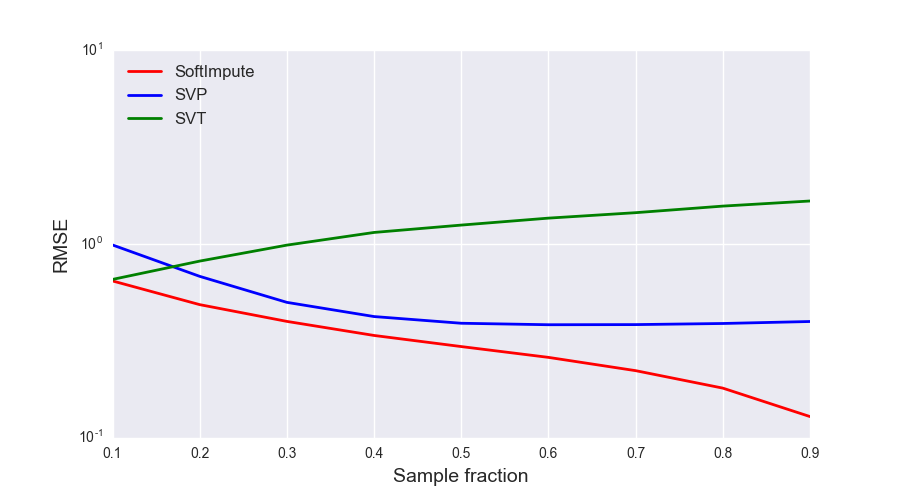
\includegraphics[width=0.8\linewidth]{./../results/real/exper_1/real_nsamp_rmse.png}
	\end{figure}
\end{frame}
%--------------------------------------------------------------------------------
\begin{frame}{Assessment data}
	\begin{figure}[h]
		\centering
		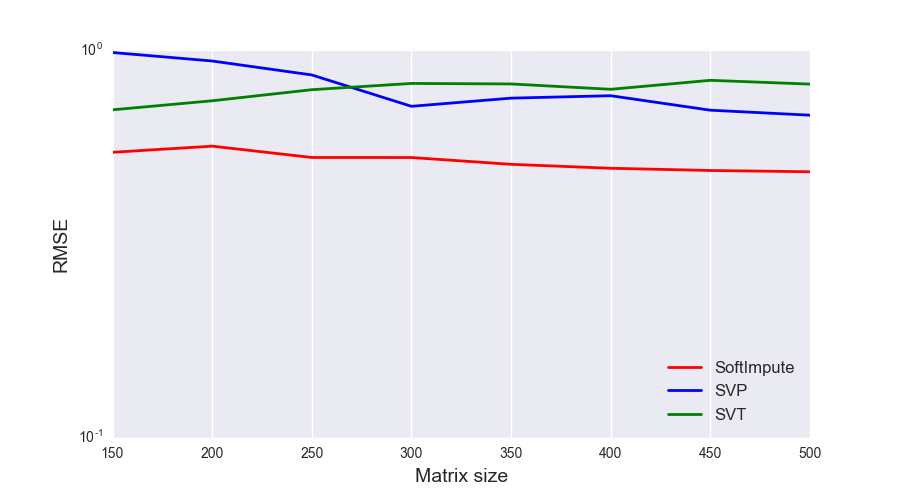
\includegraphics[width=0.8\linewidth]{./../results/real/exper_3/real_size_rmse.png}
	\end{figure}
\end{frame}
%--------------------------------------------------------------------------------

\end{document} 